%% Преамбула TeX-файла

% 1. Стиль и язык
\documentclass[draft,liberation]{G7-32}

% Остальные стандартные настройки убраны в preamble.inc.tex.
\sloppy

% Настройки стиля ГОСТ 7-32
% Для начала определяем, хотим мы или нет, чтобы рисунки и таблицы нумеровались в пределах раздела, или нам нужна сквозная нумерация.
\EqInChapter % формулы будут нумероваться в пределах раздела
\TableInChapter % таблицы будут нумероваться в пределах раздела
\PicInChapter % рисунки будут нумероваться в пределах раздела

% Добавляем гипертекстовое оглавление в PDF
\usepackage[
bookmarks=true, colorlinks=true, unicode=true,
urlcolor=black,linkcolor=black, anchorcolor=black,
citecolor=black, menucolor=black, filecolor=black,
]{hyperref}

\AfterHyperrefFix

\usepackage{microtype}% полезный пакет для микротипографии, увы под xelatex мало чего умеет, но под pdflatex хорошо улучшает читаемость

% Тире могут быть невидимы в Adobe Reader
\ifInvisibleDashes
\MakeDashesBold
\fi

\usepackage{graphicx}   % Пакет для включения рисунков

% С такими оно полями оно работает по-умолчанию:
% \RequirePackage[left=20mm,right=10mm,top=20mm,bottom=20mm,headsep=0pt,includefoot]{geometry}
% Если вас тошнит от поля в 10мм --- увеличивайте до 20-ти, ну и про переплёт не забывайте
\geometry{ignorefoot}% считать от нижней границы текста


% Пакет Tikz
\usepackage{tikz}
\usetikzlibrary{arrows,positioning,shadows}

% Произвольная нумерация списков.
\usepackage{enumerate}

% ячейки в несколько строчек
\usepackage{multirow}

% itemize внутри tabular и выравнивание таблиц
\usepackage{paralist,array,tabularx,tabulary}
\newcolumntype{C}{>{\centering\arraybackslash}X}

%\setlength{\parskip}{1ex plus0.5ex minus0.5ex} % разрыв между абзацами
\setlength{\parskip}{1ex} % разрыв между абзацами
\usepackage{blindtext}

% Центрирование подписей к плавающим окружениям
%\usepackage[justification=centering]{caption}


% Настройки листингов.
\ifPDFTeX
% 8 Листинги

\usepackage{listings}

% Значения по умолчанию
\lstset{
  basicstyle= \footnotesize,
  breakatwhitespace=true,% разрыв строк только на whitespacce
  breaklines=true,       % переносить длинные строки
%   captionpos=b,          % подписи снизу -- вроде не надо
  inputencoding=koi8-r,
  numbers=left,          % нумерация слева
  numberstyle=\footnotesize,
  showspaces=false,      % показывать пробелы подчеркиваниями -- идиотизм 70-х годов
  showstringspaces=false,
  showtabs=false,        % и табы тоже
  stepnumber=1,
  tabsize=4,              % кому нужны табы по 8 символов?
  frame=single
}

% Стиль для псевдокода: строчки обычно короткие, поэтому размер шрифта побольше
\lstdefinestyle{pseudocode}{
  basicstyle=\small,
  keywordstyle=\color{black}\bfseries\underbar,
  language=Pseudocode,
  numberstyle=\footnotesize,
  commentstyle=\footnotesize\it
}

% Стиль для обычного кода: маленький шрифт
\lstdefinestyle{realcode}{
  basicstyle=\scriptsize,
  numberstyle=\footnotesize
}

% Стиль для коротких кусков обычного кода: средний шрифт
\lstdefinestyle{simplecode}{
  basicstyle=\footnotesize,
  numberstyle=\footnotesize
}

% Стиль для BNF
\lstdefinestyle{grammar}{
  basicstyle=\footnotesize,
  numberstyle=\footnotesize,
  stringstyle=\bfseries\ttfamily,
  language=BNF
}

% Определим свой язык для написания псевдокодов на основе Python
\lstdefinelanguage[]{Pseudocode}[]{Python}{
  morekeywords={each,empty,wait,do},% ключевые слова добавлять сюда
  morecomment=[s]{\{}{\}},% комменты {а-ля Pascal} смотрятся нагляднее
  literate=% а сюда добавлять операторы, которые хотите отображать как мат. символы
    {->}{\ensuremath{$\rightarrow$}~}2%
    {<-}{\ensuremath{$\leftarrow$}~}2%
    {:=}{\ensuremath{$\leftarrow$}~}2%
    {<--}{\ensuremath{$\Longleftarrow$}~}2%
}[keywords,comments]

% Свой язык для задания грамматик в BNF
\lstdefinelanguage[]{BNF}[]{}{
  morekeywords={},
  morecomment=[s]{@}{@},
  morestring=[b]",%
  literate=%
    {->}{\ensuremath{$\rightarrow$}~}2%
    {*}{\ensuremath{$^*$}~}2%
    {+}{\ensuremath{$^+$}~}2%
    {|}{\ensuremath{$|$}~}2%
}[keywords,comments,strings]

% Подписи к листингам на русском языке.
\renewcommand\lstlistingname{Листинг}
\renewcommand\lstlistlistingname{Листинги}

\else
\usepackage{local-minted}
\fi

% Полезные макросы листингов.
% Любимые команды
\newcommand{\Code}[1]{\textbf{#1}}


% Стиль титульного листа и заголовки
%\NirEkz{Экз. 3}             % Раскоментировать если не требуется
%\NirGrif{Секретно}                % Наименование грифа

%\gosttitle{Gost7-32}       % Шаблон титульной страницы, по умолчанию будет ГОСТ 7.32-2001, 
% Варианты GostRV15-110 или Gost7-32 

\NirOrgLongName{\small
МИНОБРНАУКИ РОССИИ\\
Федеральное государственное автономное образовательное учреждение высшего образования\\
<<Национальный исследовательский университет\\<<Московский институт электронной техники>>\\
~\\
Кафедра информатики и программного обеспечения вычислительных систем
}                   %% Полное название организации

%\NirUdk{УДК № 378.14}
%\NirGosNo{№ госрегистрации 01970006723}
%\NirInventarNo{Инв. № ??????}

%\NirConfirm{Согласовано}                  % Смена УТВЕРЖДАЮ
\NirBossStamp{}


\NirReportName{Фаткуллин Осип Андреевич}   % Можно поменять тип отчета
\NirAbout{} %Можно изменить о чем отчет

%\NirPartNum{Часть}{1}                      % Часть номер

\NirBareSubject{}                  % Убирает по теме если раскоментить

% \NirIsAnnotacion{АННОТАЦИОННЫЙ }         %% Раскомментируйте, если это аннотационный отчёт
%\NirStage{промежуточный}{Этап \No 1}{} %%% Этап НИР: {номер этапа}{вид отчёта - промежуточный или заключительный}{название этапа}
%\NirStage{}{}{} %%% Этап НИР: {номер этапа}{вид отчёта - промежуточный или 

\Nir{Бакалаврская работа\\по направлению 09.03.04 <<Программная инженерия>>}

\NirSubject{Разработка мобильного приложения сопровождения учебного\\
процесса студентов в системе ОРИОКС} % Наименование темы
%\NirFinal{}                        % Заключительный, если закоментировать то промежуточный
%\finalname{итоговый}               % Название финального отчета (Заключительный) 
%\NirCode{Шифр\,---\,САПР-РЛС-ФИЗТЕХ-1} % Можно задать шифр как в ГОСТ 15.110
\NirCode{Шифр МП СУПС}

\NirManager{Руководитель,\\доцент, к.п.н.}{Е.Л. Федотова~~~~} %% Название руководителя
\NirIsp{Студент}{О.А. Фаткуллин} %% Название руководителя

%\NirYear{1999}%% если нужно поменять год отчёта; если закомментировано, ставится текущий год
\NirTown{Москва}                           %% город, в котором написан отчёт



\begin{document}

    \frontmatter % выключает нумерацию ВСЕГО; здесь начинаются ненумерованные главы: реферат, введение, глоссарий, сокращения и прочее.

    \maketitle %создает титульную страницу


    %\begin{executors}
    %\personalSignature{Первый исполнитель}{ФИО}
    %
    %\personalSignature{Второй исполнитель}{ФИО}
    %\end{executors}


    %\listoffigures                         % Список рисунков

    %\listoftables                          % Список таблиц

    %\NormRefs % Нормативные ссылки
    % Команды \breakingbeforechapters и \nonbreakingbeforechapters
    % управляют разрывом страницы перед главами.
    % По-умолчанию страница разрывается.

    % \nobreakingbeforechapters
    % \breakingbeforechapters

    % Также можно использовать \Referat, как в оригинале
\begin{abstract}

    Отчет содержит \pageref{LastPage}\,стр.%
    \ifnum \totfig >0
    , \totfig~рис.%
    \fi
    \ifnum \tottab >0
    , \tottab~табл.%
    \fi
    %
    \ifnum \totbib =1
    , \totbib~источник%
    \else
    \ifnum \totbib >1
    \ifnum \totbib <5
    , \totbib~источника%
    \else
    , \totbib~источников%
    \fi
    \fi
    \fi
    %
    \ifnum \totapp >0
    , \totapp~прил.%
    \fi


    Это пример каркаса расчётно-пояснительной записки, желательный к использованию в РПЗ проекта по курсу РСОИ
    \nocite{*}.

    Данный опус, как и более новые версии этого документа, можно взять по адресу (\url{https://github.com/latex-g7-32/latex-g7-32}).

    Текст в документе носит совершенно абстрактный характер.

\end{abstract}

%%% Local Variables: 
%%% mode: latex
%%% TeX-master: "rpz"
%%% End: 


    \tableofcontents

    \printnomenclature % Автоматический список сокращений

    \Introduction
\Abbrev{МП СУПС}{мобильное приложение сопровождения учебного процесса студентов в системе ОРОИКС}
\hyphenation{МИЭТе}
В современных учебных заведениях всё чаще практикуют использование систем сопровождения учебного процесса, которые позволяют учащимся видеть свои оценки, получать домашние задания, узнавать о событиях учебного процесса.
\Abbrev{ОРИОКС}{организация распределенного информационного обмена в корпоративных средах}
В МИЭТе такой системой является ОРИОКС (Организация Распределенного Информационного Обмена в Корпоративных Средах).

Слабым местом ОРИОКС является невозможность оперативного оповещения учащихся о событиях учебного процесса.
\Define{Веб-приложение}{клиент-серверное приложение, в котором клиент взаимодействует с сервером при помощи браузера, а за сервер отвечает — веб-сервер}
Это обусловлено тем, что ОРИОКС представляет из себя веб-приложение и подразумевает регулярное посещение через браузер.
Если же студент долгое время не заходит в систему, что бывает довольно часто, то он может пропустить информацию о важных событиях, например о пересдачах.
Так же, в ОРИОКС невозможна установка напоминаний о предстоящих событиях.

Еще одна проблема веб-приложений – неудобство использования на мобильных
устройствах.
Большая часть студентов посещает ОРИОКС именно с мобильных
устройств, и, хотя, дизайн сайта оптимизирован для работы на небольших экранах, всё же мобильные устройства накладывают свои ограничения.
\Abbrev{ПК}{персональный компьютер}
Скорость интернет соединения, чаще всего, ниже чем на стационарных ПК, кроме того, соединение может часто разрываться, что приводит к дискомфорту
при использовании веб-приложения, т.к.\ для каждой страницы браузер должен
загрузить, помимо данных, разметку и таблицу стилей.


\Define{Мобильное приложение}{программное приложение, предназначенное для работы на смартфонах или планшетных компьютерах}
\Abbrev{API}{application programming interface "--- внешний интерфейс взаимодействия с приложением}
Все эти недостатки можно устранить, создав мобильное приложение, которое будет получать данные от сервера ОРИОКС через API).
Это позволит запрашивать и получать только ту информацию, которая нужна для работы приложения в конкретный момент времени, так как приложению не нужно скачивать таблицу стилей и разметку.
В виду малого потребления трафика приложение сможет работать на смартфоне в фоновом режиме и отображать уведомления и напоминания в тот момент когда они только пришли.

Удобство работы с системой ОРИОКС при нестабильном интернет соединении тоже повысится за счёт меньшего объёма пересылаемых данных.
\Define{Кэширование}{один из способов оптимизации приложений. Заключается в том, чтобы сохранять на некоторое время и переиспользовать результаты медленных операций.}
Кроме того, приложение может кэшировать данные и использовать их даже при отсутствии интернет соединения.

На данный момент нет ни одного приложения работающего с ОРИОКС через API, обладающего полным функционалом и предоставляющего возможности push-уведомлений, поэтому задача является актуальной.
Целью данной работы является создание такого приложения, чтобы повысить оперативность оповещения студентов о событиях учебного процесса.

Задачи выпускной квалификационной работы:
\begin{itemize}
  \item сравнительный анализ существующих программных решений;
  \item выбор платформы;
  \item выбор языка и среды программирования;
  \item разработка алгоритма;
  \item разработка схемы данных;
  \item разработка пользовательского интерфейса;
  \item отладка и тестирование;
  \item разработка руководства оператора.
\end{itemize}

Пояснительная записка состоит из введения, исследовательского, конструкторского и технологического разделов, заключения, списка использованных источников и трёх приложений.

Исследовательский раздел содержит обзор существующих решений, исследование структуры ОРИОКС, описание входных и выходных данных, постановку целей и задач.
Конструкторский раздел содержит обзор и выбор языка программирования, среды разработки, выбор стека технологий, описание алгоритма работы, схему данных и макеты пользовательского интерфейса.
Технологический раздел включает в себя описания применяемых технологий, нюансы разработки под Android, описание процессов сборки, публикации, тестирования, отладки и сопровождения.

В приложении~\ref{ch:appendix1} содержится техническое задание на разработку МП СУПС.
Приложение~\ref{ch:appendix2} содержит фрагменты исходного кода приложения.
В приложении~\ref{ch:appendix3} "--- руководство оператора.


    \mainmatter % это включает нумерацию глав и секций в документе ниже

    \chapter{Исследовательский раздел}
\label{ch:research}
%
% % В начале раздела  можно напомнить его цель
%

\section{Актуальность разработки мобильного приложения}
\label{sec:whyApp}

Мобильные приложения могут быть инструментом для быстрой доставки информации, чего нельзя добиться при помощи обычного веб-приложения.

Индустрия мобильных устройств очень быстро развивается.
На смену старым устройствам приходят более новые, современные и обладающие большим спектром возможностей.
Количество пользователей с каждым годом растёт.
сейчас смартфоны есть почти у всех студентов и они редко с ними расстаются надолго.
Конечно, важную роль играет программная составляющая "--- мобильные приложения.
Они существуют совершенно разной направленности:
\begin{itemize}
  \item развлекательные (игры, музыкальные и видео проигрыватели и т.д.);
  \item коммуникационные (мессенджеры, навигаторы и т.д.);
  \item справочные (словари, базы знаний);
  \item прикладные (все остальные от графического редактора до калькулятора).
\end{itemize}

Кроме того, популярность мобильных приложений повлекла за собой появление мощных инструментов разработки, большого количества библиотек и фреймворков, что, в свою очередь, сделало разработку приложений быстрой, лёгкой и продуктивной.


\section{Обзор аналогичных решений}
\label{sec:analogs}
Был произведен поиск существующих решений в Windows Phone Store, Google Play, Apple App Store, на GitHub, и было найдено 3 аналога.
К ним можно, так же, добавить сам сайт ОРИОКС.

Рассмотрим преимущества и недостатки каждого решения по отдельности.
В качестве критериев будем брать:
\begin{itemize}
  \item способ получения данных;
  \item возможность push-уведомлений;
  \item возможность просмотра расписания;
  \item возможность просмотра текущих предметов;
  \item возможность просмотра успеваемости;
  \item возможность просмотра списка долгов;
  \item возможность просмотра списка пересдач;
  \item наличие графического интерфейса;
  \item оффлайн доступ.
\end{itemize}
\Define{Push-уведомления}{способ рассылки уведомлений. У конечного пользователя такие уведомления выглядят как небольшое всплывающее окошко на экране телефона или в браузере}

\begin{figure}[ht]
  \centering
  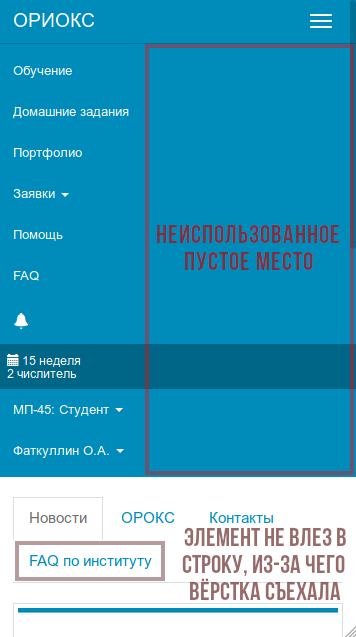
\includegraphics[width=\textwidth/2]{inc/img/orioks_mobile.png}
  \caption{Главная страница ОРИОКС с открытым меню}
  \label{fig:orioksMobile}
\end{figure}

\subsection{Сайт ОРИОКС}
\label{subsec:orioks}

\Define{Платформа}{среда выполнения, в которой должен выполняться фрагмент программного обеспечения или объектный модуль с учётом накладываемых средой ограничений и предоставляемых возможностей}
\Define{Браузер}{программное обеспечение для просмотра информации в сети Интернет}
Платформа: Браузер.

\Abbrev{БД}{база данных}
Из плюсов: cайт ОРИОКС получает информацию напрямую из БД.
Это позволяет позволяет запрашивать только ту информацию, которая нужна в данный момент для отображения страницы.
Можно, так же, отметить наличие всех перечисленных выше возможностей, за исключением просмотра расписания (но его можно посмотреть на сайте МИЭТ)~\cite{orioks}.
Графический интерфейс присутствует, но не полностью адаптирован для мобильных устройств, то есть в некоторых местах элементы интерфейса не помещаются на экране, а в других "--- наоборот слишком много неиспользованного места (см.~рис.~\ref{fig:orioksMobile}).

\Abbrev{HTML}{hypertext markup language "--- язык гипертекстовой разметки}
К минусам можно отнести отсутствие push-уведомлений, невозможность просмотра информации без интернет соединения и необходимость загружать таблицы стилей и HTML разметку для просмотра страницы.

\begin{figure}[ht]
  \centering
  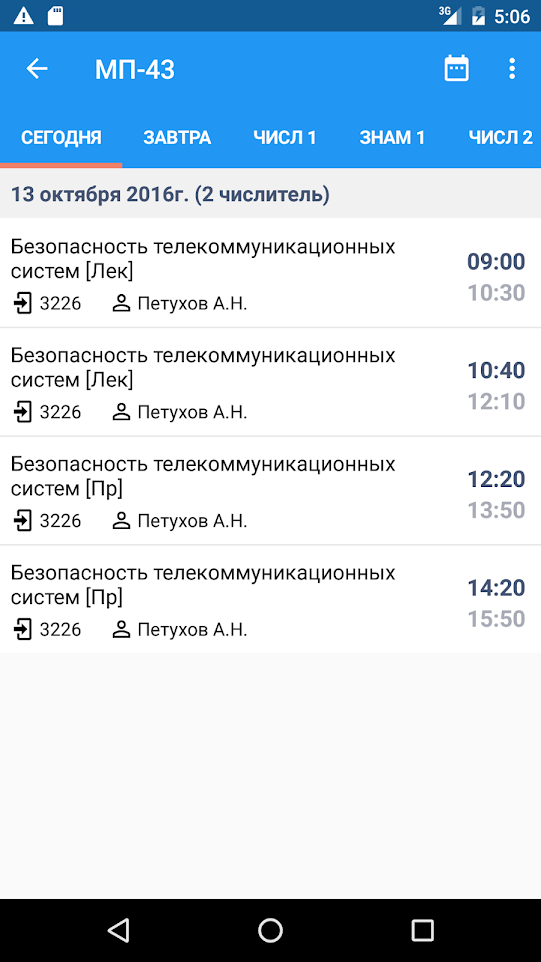
\includegraphics[width=\textwidth/2]{inc/img/miet_schedule.png}
  \caption{Экран расписания в приложении ``Расписание для МИЭТ''}
  \label{fig:mietSchedule}
\end{figure}

\subsection{Приложение ``Расписание для МИЭТ''}
\label{subsec:appMietSchedule}
Платформа: Android.
Дополнительная информация: около тысячи установок;
рейтинг на Google Play "--- 4.7 из 5;
дата последнего обновления "--- 22.04.2018.

Приложение предназначено для просмотра новостей МИЭТ и расписания любой группы с возможностью скачать его и использовать в оффлайн-режиме.
Раньше присутствовал функционал просмотра успеваемости, но из-за изменений на сайте ОРИОКС этот функционал стал недоступен~\cite{market:mietSchedule}.

Получение расписания реализовано через API, это плюс.
Для получения текущей успеваемости использовался синтаксический анализ сайта.
При таком подходе любое изменение в таблице стилей или HTML разметке сайта приводит к неработоспособности приложения, что и случилось.

Из требуемых возможностей присутствует просмотр и кэширование расписания, это позволяет просматривать его без интернет-соединения
Просмотр текущих предметов, успеваемости, списка долгов и пересдач невозможен.

Графический интерфейс присутствует, но не соответствует требованиям Material Design.
Например, слишком маленькие отступы от краёв экрана (см.~рис.~\ref{fig:mietSchedule}).

\begin{figure}[ht]
  \centering
  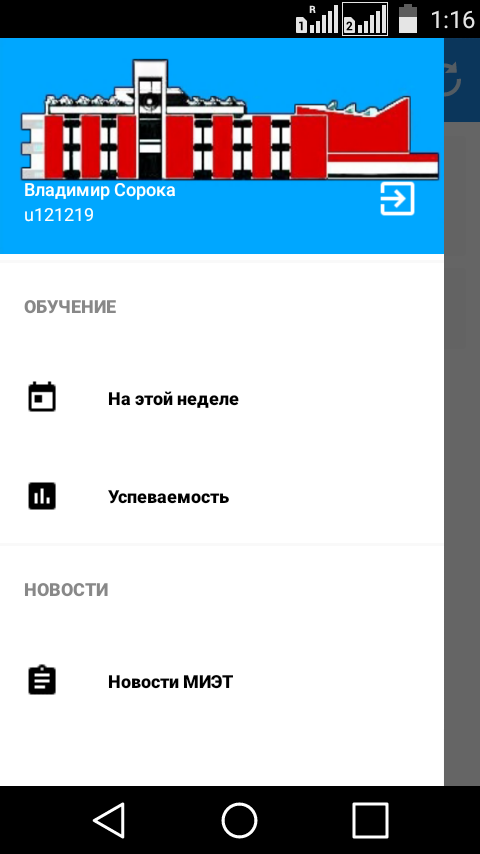
\includegraphics[width=\textwidth/2]{inc/img/orioks_live.png}
  \caption{Главный экран с открытым меню в приложении ``Ориокс Live''}
  \label{fig:orioksLive}
\end{figure}

\subsection{Приложение ``ОРИОКС Live''}
\label{subsec:appOrioksLive}
Платформа: Android.
Дополнительная информация: около тысячи установок;
рейтинг на Google Play "--- 3.9 из 5;
дата последнего обновления "--- 30.09.2015.

Приложение предназначено для просмотра успеваемости, списка контрольных мероприятий и информации о преподавателях~\cite{market:orioksLive}.

Данные получаются при помощи непубличного программного интерфейса, но интерфейс был удалён, т.к. был сделан неофициально и работа с ОРИОКС стала невозможна.
Приложение не обновлялось с 2015 года и на данный момент не работает.

Заявленный функционал проверить не удалось из-за невозможности авторизации, поэтому все эти возможности отметим как отсутствующие.
Рабочей осталась только возможность просмотра новостей.

Графический интерфейс присутствует, но не соответствует требованиям Material Design.
Неправильные отступы, слишком контрастные цвета (см.~рис.~\ref{fig:orioksLive}).

\begin{figure}[ht]
  \centering
  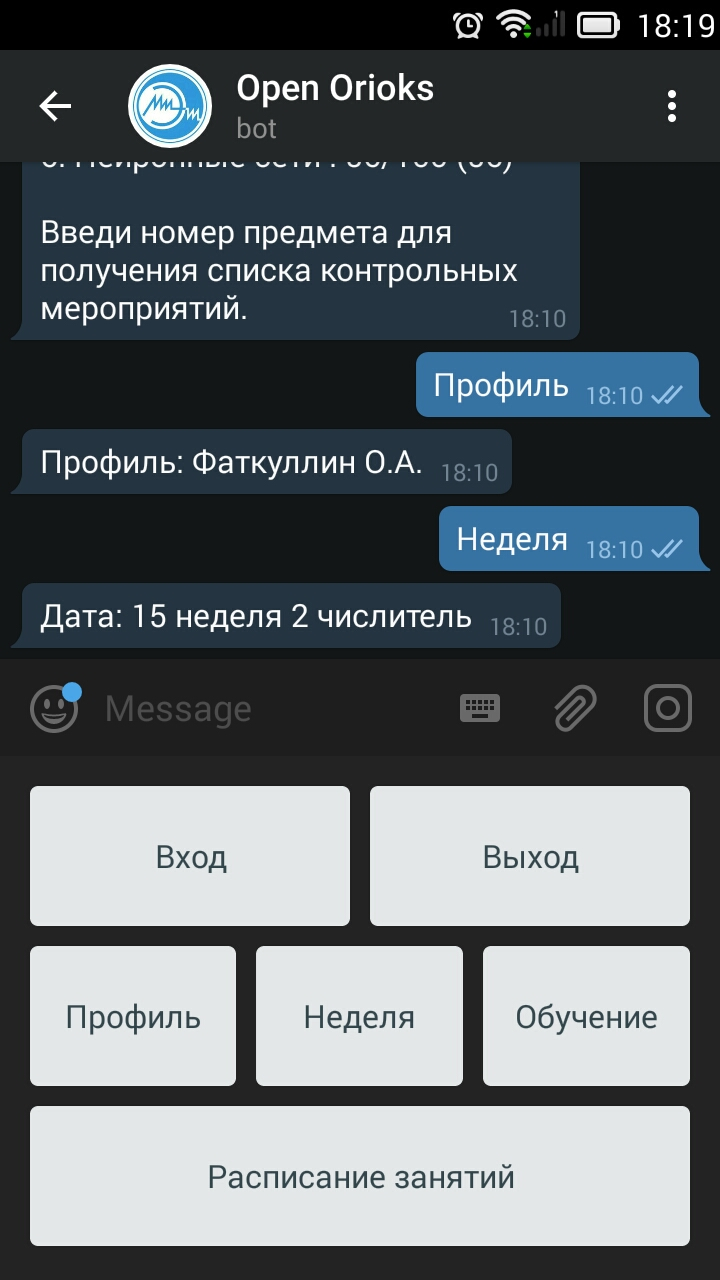
\includegraphics[width=\textwidth/2]{inc/img/open_orioks.jpg}
  \caption{Интерфейс управления Telegram-ботом ``Open Orioks''}
  \label{fig:openOrioks}
\end{figure}

\subsection{Telegram-бот ``Open Orioks''}
\label{subsec:botOpenOrioks}
Платформа: Telegram.
Дополнительная информация: последнее обновление "--- 12.10.2017.

Бот позволяет просматривать расписание на день, текущую успеваемость и список контрольных мероприятий по каждому предмету.

Для получения данных используется синтаксический анализ (как и в пункте~\ref{subsec:appMietSchedule}), но за счёт того, что данные всех студентов обновляются раз в полчаса и сохраняются в хранилище бота, скорость получения данных конечным пользователем сравнима со скоростью получения данных из БД~\cite{github:openOrioks}.

Собственного графического интерфейса нет.
Взаимодействие с ботом производится через текстовые сообщения в мессенджере Telegram.
Использование при отсутствии интернета невозможно, но можно просматривать предыдущие ответы бота, что можно считать частичным кэшированием.

По итогом обзора аналогичных решений была построена таблица~\ref{tab:analogs}.
Как видно из таблицы, нет ни одного решения, которое бы соответствовало всем необходимым параметрам, что еще раз доказывает актуальность задачи.

\begin{table}[ht]
  \caption{Сравнение аналогичных решений}
  \label{tab:analogs}
  \small
  \begin{tabularx}{\textwidth}{|>{\raggedright}m{.203\textwidth}|>{\hsize=.9\hsize}C|>{\hsize=1.2\hsize}C|C|>{\hsize=.9\hsize}C|c|}
    \hline
    Критерий & Сайт ОРИОКС~\cite{orioks} & Приложение ``Расписание для МИЭТ''~\cite{market:mietSchedule} & Приложение ``ОРИОКС Live''~\cite{market:orioksLive} & Бот ``Open Orioks''~\cite{github:openOrioks} & МП СУПС \\
    \hline
    Скорость получения информации & Средняя & Высокая & Низкая  & Средняя & Высокая \\
    \hline
    Push-уведомления              & $-$     & $-$     & $-$     & $+$     & $+$     \\
    \hline
    Расписание                    & $\pm$   & $+$     & $-$     & $\pm$   & $+$     \\
    \hline
    Текущие предметы              & $+$     & $-$     & $-$     & $+$     & $+$     \\
    \hline
    Успеваемость                  & $+$     & $-$     & $-$     & $+$     & $+$     \\
    \hline
    Долги                         & $+$     & $-$     & $-$     & $-$     & $+$     \\
    \hline
    Пересдачи                     & $+$     & $-$     & $-$     & $-$     & $+$     \\
    \hline
    Графический интерфейс         & $+$     & $-$     & $-$     & $-$     & $+$     \\
    \hline
    Оффлайн доступ                & $-$     & $+$     & $-$     & $\pm$   & $+$     \\
    \hline
  \end{tabularx}
  \caption*{
    \small
    \raggedright
    $+$ -- указанная возможность присутствует\\
    $\pm$ -- указанная возможность частично присутствует\\
    $-$ -- указанная возможность отсутствует
  }
\end{table}

В приложении ``Расписание для МИЭТ'' есть кэширование, но работает оно только для расписания, так как остальные функции недоступны.
Только Telegram-бот ``Open Orioks'' предоставляет возможность push-уведомлений, но не обладает всеми требуемыми возможностями, т.к.\ при увеличении количества выполняемых задач, бот становится неудобен в использовании.


\section{Обзор мобильных платформ}
\label{sec:platforms}
Смартфоны, в виде, похожем на нынешний, появились в 2007 году, когда Стив Джобс на выставке ``Macworld Conference \& Expo'' показал миру iPhone.
Все существующие телефоны мгновенно стали устаревшими.
Рынок смартфонов был практически пуст и было понятно, что один iPhone c iOS его не покроет.
В Google в это время только думали о выпуске своего телефона, но о смартфоне речи не шло.

\Abbrev{ОС}{операционная система}
За четыре года до этого, в 2003 году, Энди Рубин, Ник Сир, Крис Уайт и Рич Майнер решили создать операционную систему для носимых устройств, которые могли бы подстраиваться под нужды пользователя.
Они основали компанию Android Inc.\ и назвали свою операционную систему Android.
Никто тогда не оценил этот стартап и в 2005 году компания была на грани банкротства, но Энди Рубин смог убедить Google, которая занималась скупкой инновационных проектов, в том, что у Android есть будущее.
Так и оказалось.

В 2007 году Google вспоминает, что они покупали стартап, направленный на разработку операционной системы для переносных устройств.
Команда Android была только рада заняться разработкой ОС, но нужно было найти производителя смартфонов, который был бы готов выпустить на рынок устройство с совершенно новой ОС.
У Nokia уже была своя ОС "--- Symbian.
Motorola в это время была ослеплена успехом Razr и вряд ли обратила бы внимание на Android.
Оставались еще LG и HTC, но LG уже решили развивать Windows Mobile вместе с Microsoft, поэтому выбор пал на HTC\@.
HTC была рада сотрудничеству с большой компанией и могла обеспечить быстрый выпуск прототипов устройств.
В 2007--2008 году Google и HTC интенсивно работали над первым смартфоном на базе Android "--- HTC Dream.
22 октября 2008 года устройство уже поступило в продажу.

\todo{Добавить инфографику с историей развития мобильных платформ.}

В 2009 году Microsoft тоже попыталась выйти на рынок смартфонов и выпустила Windows Phone 7.
Проект оказался неудачным, своего рода ``мобильная Vista''.
Продажи устройств на Windows Mobile и Symbian упали и остались только две развивающиеся ОС "--- Android и iOS\@.
Apple не позволяла сторонним компаниям использовать iOS, поэтому все взгляды обратились  на Android.

\begin{figure}[ht]
  \centering
  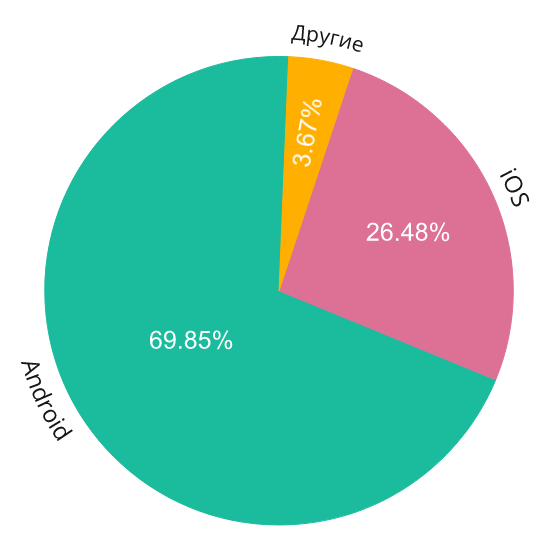
\includegraphics[width=\textwidth/2]{inc/svg/os_popularity}
  \caption{Доля устройств (данные по России)}
  \label{fig:osPopularity}
\end{figure}

Гонка Apple и Google продолжалась.
Компании улучшали свои ОС чтобы превзойти друг друга по быстродействию, безопасности, интерфейсу, функциональности, удобству использования и т.д\@.
В данный момент обе ОС достигли высокого уровня по всем направлениям, но в силу того, что Android "--- открытая система и лицензии (Apache v2 и GNU GPL v2) не запрещают устанавливать адаптировать её под любые устройства, она гораздо популярнее чем iOS\@.

Исходя из доли устройств с каждой мобильной ОС в России (см.~рис.~\ref{fig:osPopularity}), будем выбирать из двух вариантов: iOS и Android.
Разработка для iOS ведется на языке Swift или Objective-C, для работы среды разработки требуется устройство под управлением MacOS~\cite{appleDev}.
Для разработки под Android можно использовать Java или Kotlin, среда разработки не накладывает ограничений на ОС разработчика, так как доступна для Windows, Linux и MacOS~\cite{androidDev}.

\begin{table}[ht]
  \caption{Сравнение мобильных платформ}
  \label{tab:os}
  \begin{tabular*}{\textwidth}{|L|M{0.29\textwidth}|M{0.19\textwidth}|M{0.12\textwidth}|M{0.138\textwidth}|}
    \hline
    Название & Поддерживаемые языки программирования & Доля устройств (Россия)~\cite{statista:os} & Исходный код & ОС для разработки \\
    \hline
    iOS~\cite{appleDev}       & Swift, Objective-C & 26.48\% & Закрытый & MacOS \\
    \hline
    Android~\cite{androidDev} & Kotlin, Java       & 69.85\% & Открытый & GNU\textbackslash Linux, Windows, MacOS \\
    \hline
  \end{tabular*}
\end{table}

Для сравнения была составлена таблица~\ref{tab:os}.
Исходя из покрытия устройств, открытости исходного кода, ограничений на ОС для разработки и наличия опыта программирования на языках Java и Kotlin, была выбрана платформа Android.


\section{Исследование структуры ОРИОКС, концептуальная модель}
\label{sec:orioksStructure}

Функционал ОРИОКС делится на несколько частей, мы будем рассматривать только часть которая касается студентов, и говоря, например, ``инфологическая модель ОРИОКС'' будем иметь ввиду инфологическую модель студенческой части ОРИОКС\@.

На главной странице есть доступ к новостям, FAQ, портфолио, текущей успеваемости.
При открытии страницы успеваемости отображается список предметов, текущий балл по каждому из них и индикатор контрольного мероприятия (если индикатор активен, значит на этой неделе есть контрольное мероприятие по этому предмету).
Список дисциплин одинаков для всех студентов из одной группы.
Но если студент обучается по индивидуально плану, список его предметов будет отличаться.
Кроме того, у каждого студента может быть собственный список долгов, который хранится и отображается отдельно от текущих дисциплин.

Нажатие на строку предмета открывает страницу с подробной информацией, где содержится список преподавателей, форма зачёта, список ресурсов, название кафедры и список контрольных мероприятий.
Для каждого мероприятия выводится:
\begin{itemize}
  \item номер недели когда проходит мероприятие;
  \item название контрольного мероприятия;
  \item форма контроля;
  \item максимальное количество баллов;
  \item текущее количество баллов;
  \item индикатор является контрольное мероприятие обязательным или дополнительным.
\end{itemize}

Расписание не представлено в ОРИОКС, но оно есть на сайте МИЭТ.
Для каждой записи в расписании указывается:
\begin{itemize}
  \item предмет;
  \item день недели;
  \item тип недели (каждую неделю, 1/2 числитель/знаменатель);
  \item номер аудитории;
  \item номер пары;
  \item тип занятия (лабораторная работа, лекция, семинар);
  \item преподаватель.
\end{itemize}

\nocite{db}
\begin{figure}[ht]
  \centering
  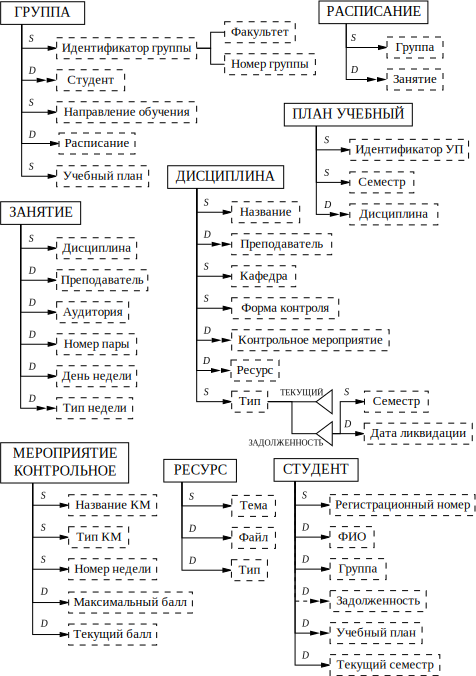
\includegraphics[width=\textwidth]{inc/svg/orioks_concept}
  \caption{Инфологическая модель ОРИОКС}
  \label{fig:orioksConcept}
\end{figure}

\begin{figure}[ht]
  \centering
  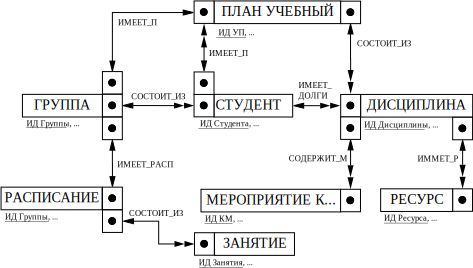
\includegraphics[width=\textwidth]{inc/svg/orioks_er}
  \caption{ER-диаграмма ОРИОКС}
  \label{fig:orioksEr}
\end{figure}

\Abbrev{ИЛМ}{инфологическая модель предметной области}
\Abbrev{ER}{entity-relationship (сущность-связь)}
Можно выделить следующие сущности: группа, студент, план на семестр, ресурс, дисциплина, контрольное мероприятие, расписание, занятие (одна запись из расписания).
Для них была построена ИЛМ (рис.~\ref{fig:orioksConcept}) и ER-диаграмма (рис.~\ref{fig:orioksEr}).


\section{Входные и выходные данные}
\label{sec:io}
В студенческой части ОРИОКС нет полей ввода, кроме формы запроса справки и формы портфолио.
Ввод осуществляется при помощи мыши и заключается в выборе элемента, о котором


\section{Постановка задачи}
\label{sec:problem}

\conclusions
\label{sec:researchConclusions}

    \chapter{Конструкторский раздел}
\label{ch:design}

\section{Выбор языка программирования}
\label{sec:language}

\section{Выбор среды разработки}
\label{sec:ide}

\section{Выбор стека технологий}
\label{sec:stack}

\section{Архитектура и алгоритм работы МП СУПС}
\label{sec:architecture}

\section{Разработка пользовательского интерфейса}
\label{sec:gui}

    \chapter{Технологический раздел}
\label{cha:impl}

В данном разделе описано изготовление и требование всячины. Кстати,
в Latex нужно эскейпить подчёркивание (писать <<\verb|some\_function|>> для \Code{some\_function}).

\ifPDFTeX
Для вставки кода есть пакет \Code{listings}. К сожалению, пакет \Code{listings} всё ещё
работает криво при появлении в листинге русских букв и кодировке исходников utf-8.
В данном примере он (увы) на лету конвертируется в koi-8 в ходе сборки pdf.

Есть альтернатива \Code{listingsutf8}, однако она работает лишь с
\Code{\textbackslash{}lstinputlisting}, но не с окружением \Code{\textbackslash{}lstlisting}

Вот так можно вставлять псевдокод (питоноподобный язык определен в \Code{listings.inc.tex}):

\begin{lstlisting}[style=pseudocode,caption={Алгоритм оценки дипломных работ}]
    def EvaluateDiplomas():
    for each student in Masters:
    student.Mark := 5
    for each student in Engineers:
    if Good(student):
    student.Mark := 5
    else:
    student.Mark := 4
\end{lstlisting}

Еще в шаблоне определен псевдоязык для BNF:

\begin{lstlisting}[style=grammar,basicstyle=\small,caption={Грамматика}]
    ifstmt -> "if" "(" expression ")" stmt |
    "if" "(" expression ")" stmt1 "else" stmt2
    number -> digit digit*
\end{lstlisting}

В листинге~\ref{lst:sample01} работают русские буквы. Сильная магия. Однако, работает
только во включаемых файлах, прямо в \TeX{} нельзя.

% Обратите внимание, что включается не ../src/..., а inc/src/...
% В Makefile есть соответствующее правило для inc/src/*,
% которое копирует исходные файлы из ../src и конвертирует из UTF-8 в KOI8-R.
% Кстати, поэтому использовать можно только русские буквы и ASCII,
% весь остальной UTF-8 вроде CJK и египетских иероглифов -- нельзя.

\lstinputlisting[language=C,caption=Пример (\Code{test.c}),label=lst:sample01]{inc/src/test.c}

\else

Для вставки кода есть пакет \texttt{minted}. Он хорош всем кроме: необходимости Python (есть во всех нормальных (нет, Windows, я не про тебя) ОС) и Pygments и того, что нормально работает лишь в \XeLaTeX.

\ifdefined\NoMinted
Но к сожалению, у вас, по-видимому, не установлен Python или pygmentize.
\else
Можно пользоваться расширенным BFN:

\begin{listing}[H]
    \begin{ebnfcode}
        letter = "A" | "B" | "C" | "D" | "E" | "F" | "G"
        | "H" | "I" | "J" | "K" | "L" | "M" | "N"
        | "O" | "P" | "Q" | "R" | "S" | "T" | "U"
        | "V" | "W" | "X" | "Y" | "Z" ;
        digit = "0" | "1" | "2" | "3" | "4" | "5" | "6" | "7" | "8" | "9" ;
        symbol = "[" | "]" | "{" | "}" | "(" | ")" | "<" | ">"
        | "'" | '"' | "=" | "|" | "." | "," | ";" ;
        character = letter | digit | symbol | "_" ;

        identifier = letter , { letter | digit | "_" } ;
        terminal = "'" , character , { character } , "'"
        | '"' , character , { character } , '"' ;

        lhs = identifier ;
        rhs = identifier
        | terminal
        | "[" , rhs , "]"
        | "{" , rhs , "}"
        | "(" , rhs , ")"
        | rhs , "|" , rhs
        | rhs , "," , rhs ;

        rule = lhs , "=" , rhs , ";" ;
        grammar = { rule } ;
    \end{ebnfcode}
    \caption{EBNF определённый через EBNF}
    \label{lst:ebnf}
\end{listing}

А вот в листинге \ref{lst:c} на языке C работают русские комменты. Спасибо Pygments и Minted за это.

\begin{listing}[H]
    \cfile{inc/src/test.c}
    \caption{Пример — test.c}
\end{listing}
\label{lst:c}

\fi
\fi
% Для вставки реального кода лучше использовать \texttt{\textbackslash lstinputlisting} (который понимает
% UTF8) и стили \Code{realcode} либо \Code{simplecode} (в зависимости от размера куска).




Можно также использовать окружение \Code{verbatim}, если \Code{listings} чем-то не
устраивает. Только следует помнить, что табы в нём <<съедаются>>. Существует так же команда \Code{\textbackslash{}verbatiminput} для вставки файла.

\begin{verbatim}
    a_b = a + b; // русский комментарий
    if (a_b > 0)
    a_b = 0;
\end{verbatim}

%%% Local Variables:
%%% mode: latex
%%% TeX-master: "rpz"
%%% End:


    \backmatter %% Здесь заканчивается нумерованная часть документа и начинаются ссылки и

    \Conclusion % заключение к отчёту

Результатом выпускной квалификационной работы является рабочее мобильное приложение для сопровождения учебного процесса студентов в системе ОРИОКС.

Мобильное приложение позволяет оповещать студентов с помощью их смартфонов о событиях учебного процесса, за счёт чего повышается удобство использования ОРИОКС и повышается оперативность получения оповещений студентами.
Целевая аудитория приложения "--- студенты МИЭТ, которые заинтересованы в упрощении взаимодействия с ОРИОКС и оповещении о событиях учебного процесса.

В рамках ВКР были решены следующие задачи:
\begin{itemize}
  \item проведено исследование предметной области;
  \item проведён сравнительный анализ существующих программных решений;
  \item выбрана платформа МП;
  \item выбран язык и среда программирования;
  \item разработан алгоритм МП;
  \item разработана схема данных МП;
  \item разработан пользовательский интерфейс МП;
  \item проведены отладка и тестирование МП;
  \item разработано руководство оператора МП.
\end{itemize}
 %% заключение


    % % Список литературы при помощи BibTeX
% Юзать так:
%
% pdflatex rpz
% bibtex rpz
% pdflatex rpz

\nocite{methodic}
\bibliographystyle{ugost2008}
\bibliography{rpz}

%%% Local Variables: 
%%% mode: latex
%%% TeX-master: "rpz"
%%% End: 



    \appendix % Тут идут приложения

    \chapter{Картинки}
\label{cha:appendix1}

\blindtext
\begin{figure}
\centering
\caption{Картинка в приложении. Страшная и ужасная.}
\end{figure}

%%% Local Variables: 
%%% mode: latex
%%% TeX-master: "rpz"
%%% End: 


    \chapter{Еще картинки}
\label{cha:appendix2}
\blindtext

\begin{figure}
\centering
\caption{Еще одна картинка, ничем не лучше предыдущей. Но надо же как-то заполнить место.}
\end{figure}

%%% Local Variables: 
%%% mode: latex
%%% TeX-master: "rpz"
%%% End: 


\end{document}
